\chapter{Rešerše používaných algoritmů}
\label{chap:reserzepouzivanychalgoritmu}
	Tato kapitola se zabývá přehledem využívaných algoritmů pro tvorbu polygonů z množiny linií. Polygonizace, tak jak jí můžeme pozorovat v různých GIS softwarech, se zpravidla neřeší jedním algoritmem, ale používají se různé algoritmy pro jednotlivé kroky polygonizace. Popíšeme zde tedy do jakých kroků lze polygonizaci rozdělit a jak jednotlivé kroky optimálně řešit. Budeme se zabývat i řešením v jednotlivých GIS softwarech.

	Polygonizaci lze nejjednodušeji rozdělit na 2 základní kroky. Jako vstupní data budeme uvažovat množinu linií, tyto linie ovšem nemusí obsahovat, v reálném použití převážně neobsahují, lomové body ve společných průsečících. Tato situace nastává především použiváme-li různé vrstvy pro tvorbu polygonů. V terminologii GIS se tyto průsečíky označují jako \textit{fuzzy}, volně přeloženo jako \textit{neostré}. Abychom mohli zahájit další krok polygonizace, je nutné tyto průsečíky doplnit. V první části se tedy budeme zabývat, jak optimálně doplnit průsečíky množin linií.
	
	Předpokládejme že množina linií je zbavená \textit{fuzzy} průsečíků, tedy každá dvojice úseček má společný nanejvýš jeden koncový bod. V takovéto situaci můžeme přistoupit k dalšímu kroku, tedy vlastní tvorbě polygonů z množiny linií. Polygony, které hledáme, musí splňovat podmínku, že žádný námi vytvořený polygon nemůže být rozdělen jakoukoliv linií na více menších polygonů. Pro řešení tvorby polygonů se často využívá grafových algoritmů.
	
\begin{figure}[h]
    \centering % <-- added
\begin{subfigure}{0.5\textwidth}
  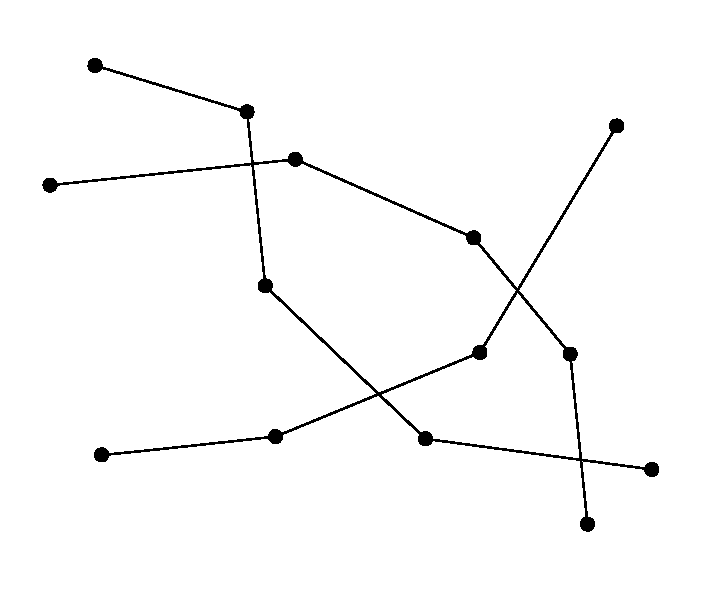
\includegraphics[width=\linewidth]{./pictures/5/fuzzy_1.pdf}
  \caption{Množina linií s fuzzy průsečíky}
  \label{fig:2-fuzzy_1}
\end{subfigure}\hfil % <-- added
\begin{subfigure}{0.5\textwidth}
  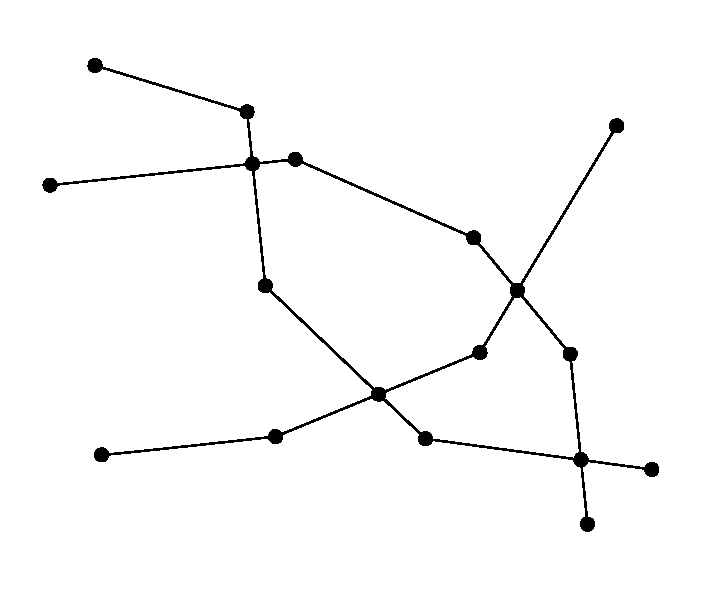
\includegraphics[width=\linewidth]{./pictures/5/fuzzy_2.pdf}
  \caption{Množina linií doplněná o průsečíky}
  \label{fig:2-fuzzy_2}
\end{subfigure}\hfil % <-- added
\begin{subfigure}{0.5\textwidth}
  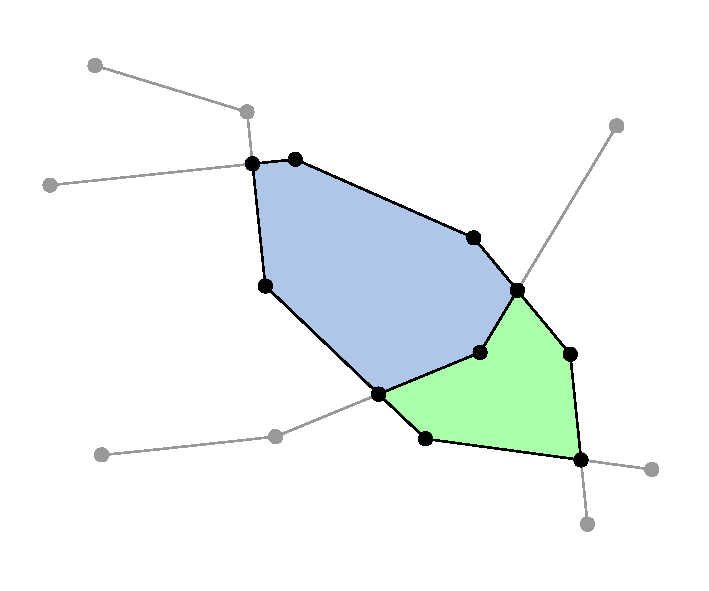
\includegraphics[width=\linewidth]{./pictures/5/fuzzy_3.pdf}
  \caption{Vytvořené polygony}
  \label{fig:2-fuzzy_2}
\end{subfigure}\hfil % <-- added
\caption{Znázornění postupu polygonizace}
\end{figure}

\section{Výpočet průsečíků množiny linií}
Výpočet všech průsečíků množin linií lze provést snadno, testováním všech úseček se všemi. Tímto postupem ovšem zjevně dosáhneme složitosti $\mathcal{O}(N^2)$ kde $N$ je počet úseček. Pro výpočet průsečíků lze ovšem využít i algoritmus s časovou náročnosti $\mathcal{O}(n\log{}n)$, známý také jako Bentley–Ottmannův algoritmus \cite{bentley1979algorithms}.

\subsection{Vzájemná poloha dvou úseček}
Ve 2D výpočetní geometrii jsou standardně jednotlivé segmenty linie vyjádřeny počátečními a koncovými souřadnicemi. Uvažujme tedy že máme dány 2 přímky $p_1 = |S_1 E_1|$ a $p_2 = |S_2 E_2|$, kde $S_1 = [x_{S1},y_{S1}]$, $E_1 = [x_{E1},y_{E1}]$, $S_2 = [x_{S2},y_{S2}]$, $E_2 = [x_{E2},y_{E2}]$ a potřebujeme provést test, zda se dané přímky protínají či nikoliv, můžeme použít takzvaný \textit{Half-Plane} test, tedy test, který určuje zda bod leží v pravé či levé polorovině od přímky. Tento test zopakujeme celkem čtyřikrát a to na počáteční a koncový bod druhé úsečky, abysme zjistili zda se přímky protínají. Test je založen na výpočtu orientace dvou vektorů $\vec{u}$  a $\vec{v}$, kde vektor $\vec{u}$ je směrový vektor úsečky, tedy $\overrightarrow{S_1E_1}$ a vektor $\vec{v}$ je vektor $\overrightarrow{S_1S_2}$. Po aplikaci výpočtu orientace vektorů na každý z koncových bodů jsme schopni jednoduše určit zda se dané přímky protínají. Tento postup nám ovšem nedá souřadnice samotného průsečíku.

\begin{figure}[h]
  \centering
  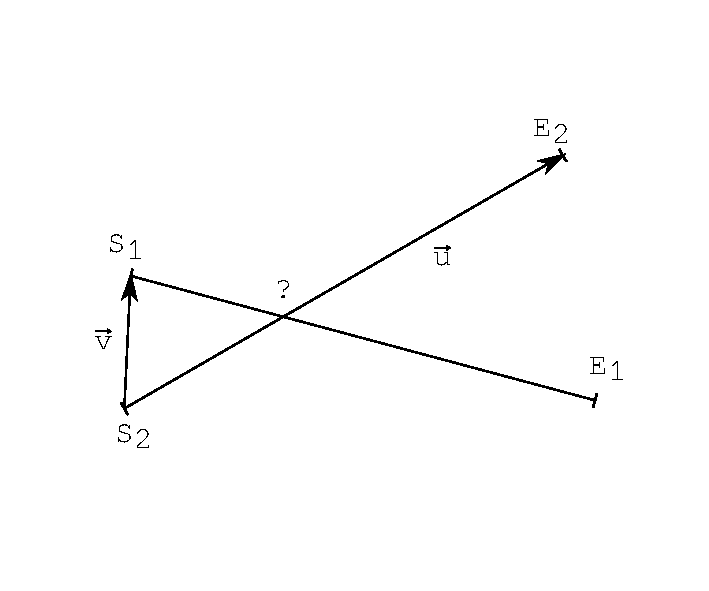
\includegraphics[width=7.5cm]{./pictures/5/half-plane_vector.pdf}
  \caption{\textit{Half-plane} test}
  \label{fig:2-half_plane_vector}
\end{figure}

\begin{figure}[h]
    \centering % <-- added
\begin{subfigure}{0.5\textwidth}
  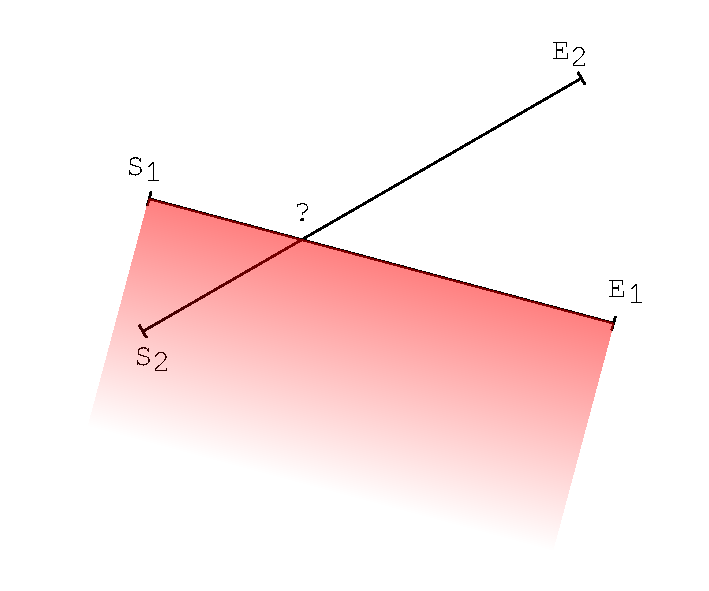
\includegraphics[width=\linewidth]{./pictures/5/half-plane_1.pdf}
  \caption{Test bodu $S_2$ k přímce $|S_1E_1|$}
  \label{fig:2-half_plane_1}
\end{subfigure}\hfil % <-- added
\begin{subfigure}{0.5\textwidth}
  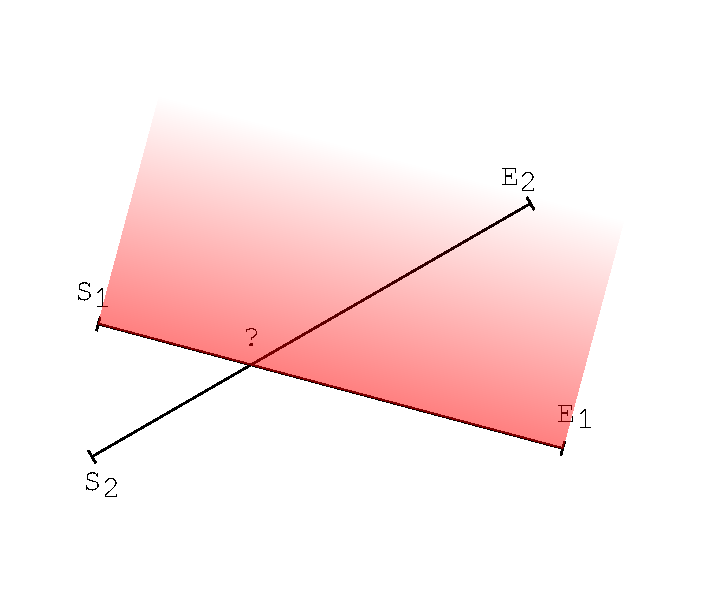
\includegraphics[width=\linewidth]{./pictures/5/half-plane_2.pdf}
  \caption{Test bodu $E_2$ k přímce $|S_1E_1|$}
  \label{fig:2-half_plane_2}
\end{subfigure}\hfil % <-- added

\medskip
\begin{subfigure}{0.5\textwidth}
  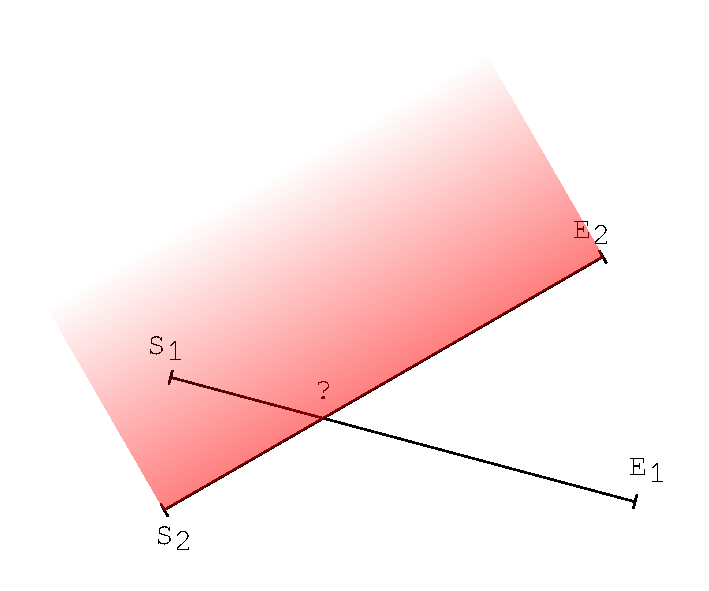
\includegraphics[width=\linewidth]{./pictures/5/half-plane_3.pdf}
  \caption{Test bodu $S_1$ k přímce $|S_2E_2|$}
  \label{fig:2-half_plane_3}
\end{subfigure}\hfil % <-- added
\begin{subfigure}{0.5\textwidth}
  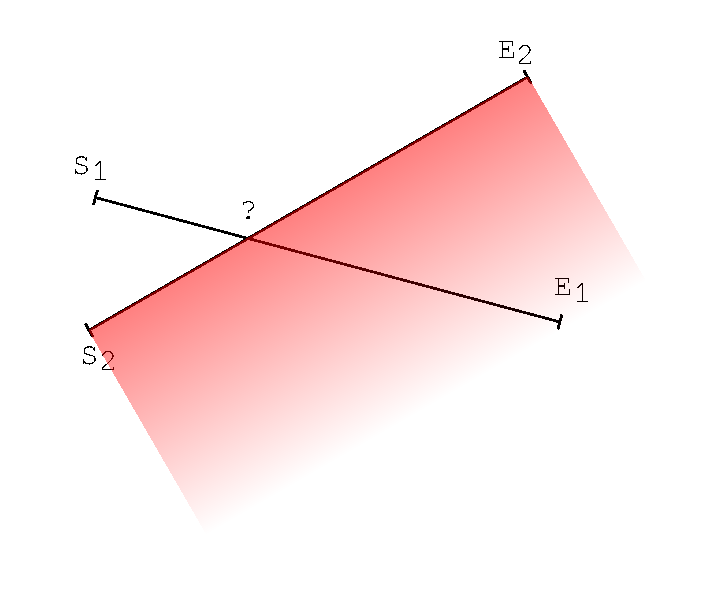
\includegraphics[width=\linewidth]{./pictures/5/half-plane_4.pdf}
  \caption{Test bodu $E_1$ k přímce $|S_2E_2|$}
  \label{fig:2-half_plane_4}
\end{subfigure}\hfil % <-- added
\caption{Grafické znázornění \textit{Half-plane} testů pro zjištění existence průsečíku}
\label{fig:2-half_plane}
\end{figure}

\subsection{Nalezení průsečíku dvou úseček}
	Pro nalezení průsečíku $P$ dvou úseček vycházíme z parametrického vyjádření přímek, jelikož obecné rovnice neumožňují pracovat s přímkami rovnoběžnými s osou y. Uvažujme tedy stejné značení bodů jako v předchozím odstavci. Nejprve je tedy nutné vyjádřit rovnici přímky z počátečního a koncového vrcholu. Pro parametrické vyjádření využijeme směrový vektor přímky a libovolný bod na přímce. Ovšem pro zjednodušení výpočtů použijeme pro přímku $p_1$ směrový vektor $\overrightarrow{S_1E_1}$ a jako bod do parametrické rovnice dosadíme $S_1$, obdobně zkonstruujeme i parametrické vyjádření přímky $p_2$. Soustava rovnic pro výpočet průsečíku $p_i$ pak tedy bude vypadat takto:
	
\begin{align*} 
P = S_1 + s \cdot \overrightarrow{S_1E_1}, \\
P = S_2 + t \cdot \overrightarrow{S_2E_2}. \\
\end{align*}

Rozepsáno podle souřadnic:

\begin{align*} 
x_P = x_{S1} + s(x_{E1} - x_{S1}), \\
y_P = y_{S1} + s(y_{E1} - y_{S1}), \\
x_P = x_{S2} + t(x_{E2} - x_{S2}), \\
y_P = y_{S2} + t(y_{E2} - y_{S2}).
\end{align*}

Pro získání průsečíku musíme nejprve ze soustavy rovnic vyjádřit parametry $s$ a $t$. To provedeme následujícím způsobem:

\begin{align*} 
s = \frac{y_{S1}(x_{S2} - x_{E2}) + y_{S2}(x_{E2} - x_{S1}) + y_{E2}(x_{S1} - x_{S2})}{(x_{E1} - x_{S1}) (y_{S2} - y_{E2})   -   (y_{E1} - y_{S1}) (x_{S2} - x_{E2})}, \\
t = \frac{y_{S1}(x_{S2} - x_{E1}) + y_{E1}(x_{S1} - x_{S2}) + y_{S2}(x_{E1} - x_{S1})}{(x_{E1} - x_{S1}) (y_{S2} - y_{E2})   -   (y_{E1} - y_{S1}) (x_{S2} - x_{E2})}.
\end{align*}


Z charakteru parametrického vyjádření přímek poté můžeme rozhodnout o vzájemné poloze úseček. Pokud parametry $s \in <0,1>, t \in <0,1>$ pak se úsečky protínají, v opačném případě se úsečky neprotínají. Je potřeba ošetřit případy kdy úsečky leží na jedné přímce.


\subsection{Bentley–Ottmannův algoritmus}
Tento algoritmus je založen na technice zvané \textit{sweep line} neboli \textit{zametací přímka}. Tato technika je již zmíněna v kapitole \ref{chap:navrhovanialgoritmu}. Hlavní myšlenka pro zrychlení algoritmu oproti metodě hrubé síly je počítat průsečíky pouze sousedních linií, tedy linií které jsou právě protnuty zametací přímkou.

prioritní fronta - seřazené body podle jedné ze souřadnic





, podle jedné ze souřadnic. Algoritmus zde nebuda více popisován jelikož je velmi dobře vysvětlen v těchto publikacích \cite{bentley1979algorithms} \cite{bayer2008algoritmy}.
% https://www.cs.princeton.edu/~rs/AlgsDS07/17GeometricSearch.pdf
% https://courses.csail.mit.edu/6.006/spring11/lectures/lec24.pdf
% https://cw.fel.cvut.cz/old/_media/courses/ae4m39vg/lectures/09-intersect.pdf





\section{Tvorba polygonů z množiny linií}
Předpokládejme že máme množinu linií doplněnou o průsečíky, tedy každá dvojice úseček v této množině sdílí nejvýše jeden koncový bod. V předchozí sekci bylo řečeno že průsečíky linií lze doplnit pomocí \textit{Bentley–Ottmannova} algoritmu v čase $\mathcal{O}(n\log{}n)$. Nyní chceme tedy v této množině linií nalézt všechny polygony, tak aby jednotlivé polygony spolu sdílely maximálně hrany a zároveň aby žádný z polygonů nemohl obsahovat jiný polygon. Takové linie jsou v podstatě reprezentací grafu. K nalezení polygonů můžeme použít tedy grafových algoritmů. 
	
\subsection{Dijkstrův algoritmus}




\section{GIS software}
Provedení polygonizace zvládá většina současně používaného GIS softwaru. Pokusíme se tedy rozebrat postupy jednotlivých nástrojů na polygonizaci.

\subsection{ArcGIS}
ArcGIS je vyvíjený společností Esri, v současné době se jedná o nejpokročilejší nástroj v oblasti GIS. Jedná se o proprietární software, u kterého 


\subsection{QGis}
QGis je nejspíše jeden z nejznámějších volných nástrojů pro práci v GIS. Je šířen pod copyleftovou  licencí \textit{GNU General Public License}, tudíž máme volný přístup ke zdrojovému kódu aplikace dostupných v online repozitářích. To nám umožňuje nahlížet do výpočetních algoritmů, které jsou v případě QGis psány v programovacím jazyce \textit{C++} a \textit{Python}, narozdíl od komerčních nástrojů, které si implementaci často chrání

\subsection{Grass GIS}

\subsection{PostGis}
